\documentclass[conference]{IEEEtran}
\IEEEoverridecommandlockouts

% --- Packages ---
\usepackage{cite}
\usepackage{amsmath,amssymb,amsfonts}
\usepackage{algorithmic}
\usepackage{graphicx}
\usepackage{textcomp}
\usepackage{xcolor}
\usepackage{booktabs}
\usepackage[hidelinks]{hyperref}
\usepackage{url}
\usepackage{tikz}
\usetikzlibrary{arrows.meta, positioning, fit, backgrounds}

\def\BibTeX{{\rm B\kern-.05em{\sc i\kern-.025em b}\kern-.08em
    T\kern-.1667em\lower.7ex\hbox{E}\kern-.125emX}}

% --- Custom commands ---
\newcommand{\TBD}[1]{\textcolor{red}{\textbf{[TBD: #1]}}}
\newcommand{\Mbytes}{\,\text{MB}}
\newcommand{\compressratio}{154{,}109\times}

\begin{document}

\title{FedSafe-Fuse: Privacy-Preserving Federated\\Medical Image Fusion with\\Spatially-Aware Conformal Uncertainty}

\author{
\IEEEauthorblockN{Furkan Yakkan}
\IEEEauthorblockA{Abdullah G\"{u}l University\\
Kayseri, T\"{u}rkiye\\
Email: furkan.yakkan@agu.edu.tr}
}

\maketitle

% =========================================================
\begin{abstract}
Federated multi-modal medical image fusion lets multiple hospitals jointly train a single fusion model without sharing raw patient images, but two unresolved gaps limit clinical deployment. First, exchanged gradients still leak training data via inversion attacks. Second, even a well-trained fusion model produces outputs that clinicians cannot calibrate per-pixel. We present \textit{FedSafe-Fuse}, a federated framework that contributes two complementary safety mechanisms, demonstrated through a lightweight Transformer--CNN fusion backbone: (1) Federated Incremental PCA (FIPCA), an orthonormal rank-$d$ projection of gradient deltas that compresses upstream traffic from 59\,MB/round (DP-SGD baseline) to 384 bytes/round (rank-32), and (2) Spatially-Aware Conformal Prediction (SACP), which uses Canny-edge region splitting to produce regional, distribution-free uncertainty thresholds with finite-sample coverage guarantees. We evaluate on both synthetic MedMNIST OrganAMNIST and \textbf{real multi-modal BraTS~2020} (T1/T2) under non-IID (K=3, T=50) federated training. The fusion task itself converges to high fidelity (SSIM~0.995 on BraTS), confirming the pipeline; FIPCA then achieves a $\compressratio$ communication reduction over DP-SGD at matched empirical privacy (DLG reconstruction SSIM~$\leq$~0.013 vs.~0.999 with raw gradients), which we complement with formal R\'enyi-DP accounting ($\varepsilon\!\approx\!6.2$ at $\delta\!=\!10^{-5}$ for the noise baseline) and a full-backbone DLG analysis. SACP attains target coverage on both datasets, with the clinically expected wider-at-boundary intervals emerging on the well-trained model. We characterise honestly the resulting tension between extreme compression and fusion quality. Code and reproducible scripts are available at \url{https://github.com/fyakkan/fedsafe-fuse}.
\end{abstract}

\begin{IEEEkeywords}
federated learning, medical image fusion, conformal prediction, differential privacy, uncertainty quantification, gradient inversion
\end{IEEEkeywords}

% =========================================================
\section{Introduction}
\label{sec:intro}

Multi-modal medical image fusion combines the structural detail of an MRI volume with the metabolic information of a PET volume into a single representation that supports diagnosis, planning, and follow-up~\cite{zhang2021ifcnn,xu2022u2fusion}. Deep fusion networks achieve strong results, but they require large, centrally aggregated multi-institutional datasets, which conflicts with patient-privacy regulations such as HIPAA and GDPR. Federated learning~\cite{mcmahan2017fedavg,li2020fedprox} addresses the data-movement constraint by training a shared model across decentralised hospital nodes, but it introduces two new clinical problems.

First, the gradients or weight deltas exchanged at each communication round are themselves leaky: Zhu \textit{et al.}~\cite{zhu2019dlg} showed that small-batch training images can be reconstructed from raw gradients with near-perfect fidelity. Standard DP-SGD~\cite{abadi2016dpsgd} mitigates this by clipping per-batch gradients and adding Gaussian noise, but the noise scale needed to block inversion attacks also destroys utility on small-batch federated medical workloads.

Second, even a fully converged fusion network produces pixel-level outputs that clinicians cannot trust uniformly. Fused images often exhibit hallucinations or boundary ambiguity, especially in out-of-distribution cases or in regions affected by cross-institutional data heterogeneity. A clinically deployable fusion model should therefore augment every fused output with a per-pixel measure of how reliable the model believes that pixel to be, and that measure should come with a distribution-free statistical guarantee.

\noindent\textbf{Contributions.} This paper presents \textit{FedSafe-Fuse}, a federated framework whose primary contributions are two privacy/uncertainty mechanisms; the fusion backbone is the vehicle through which we demonstrate and stress-test them.
\begin{itemize}
    \item \textbf{Federated Incremental PCA (FIPCA)} for gradient-level privacy: each client's weight delta is projected onto a deterministic, shared orthonormal rank-$d$ subspace before transmission. This matches DP-SGD's empirical privacy outcome (DLG reconstruction SSIM~$\leq$~0.013) while reducing upstream payload from 59.18\,MB/round to as little as 192 bytes/round at $d{=}16$ --- a $\compressratio$ reduction at rank-32.
    \item \textbf{Spatially-Aware Conformal Prediction (SACP)}: separate (1-$\alpha$)-quantile thresholds are calibrated on interior vs.~boundary pixel populations identified by Canny edge detection on the reference composite, yielding distribution-free finite-sample coverage that we validate on both synthetic and real data.
    \item \textbf{A privacy analysis that covers the deployed model and a formal DP comparison.} We run DLG against the full 4.9\,M-parameter backbone, quantitatively justify the tractable surrogate via gradient-leakage proxies that \emph{shrink} with model size, and add R\'enyi-DP accounting for the DP-SGD baseline.
    \item \textbf{Evaluation on real multi-modal BraTS~2020} (T1/T2) alongside MedMNIST, showing the federated fusion task converges to SSIM~0.995, and an honest characterisation --- including a negative result on error-feedback --- of the trade-off between extreme gradient compression and fusion quality.
    \item A complete reproducibility pipeline: every notebook, trained checkpoints, per-pixel conformity scores, the DP accountant, and CSV results are released so any reader can recompute every table without retraining.
\end{itemize}

% =========================================================
\section{Related Work}
\label{sec:related}

\noindent\textbf{Federated learning.} FedAvg~\cite{mcmahan2017fedavg} formalised parameter-averaging FL. FedProx~\cite{li2020fedprox} introduced a proximal regulariser to handle non-IID client distributions, and a wide range of subsequent works added secure aggregation, robust aggregation, or personalisation. Our implementation uses a single-process FedAvg simulator that mirrors the round structure of Flower~\cite{beutel2020flower} so the algorithm can be ported to the real Flower runtime without changing the experimental protocol.

\noindent\textbf{Medical image fusion.} IFCNN~\cite{zhang2021ifcnn} introduced a general two-stream CNN with element-wise fusion rules; we use it as a non-private federated baseline. U2Fusion~\cite{xu2022u2fusion} added unsupervised fusion via a quality-aware loss. More recent work has explored Transformer-CNN hybrids~\cite{tang2023semantic}; our backbone follows this design philosophy with a deliberately small footprint suited to federated communication budgets.

\noindent\textbf{Gradient-level privacy.} DP-SGD~\cite{abadi2016dpsgd} clips and noises per-batch gradients to achieve $(\varepsilon, \delta)$-differential privacy. The deep leakage from gradients (DLG) attack~\cite{zhu2019dlg} demonstrates that unprotected gradients leak training data with near-perfect fidelity, motivating the protections we evaluate.

\noindent\textbf{Conformal prediction.} Vovk \textit{et al.}~\cite{vovk2005alrw} established conformal methods for distribution-free prediction sets with finite-sample coverage guarantees. Angelopoulos \textit{et al.}~\cite{angelopoulos2022cv} extended conformal methods to dense prediction tasks in computer vision. To our knowledge no prior work has combined federated training, gradient-level projection privacy, and spatially-aware conformal calibration in the medical-fusion setting.

% =========================================================
\section{Methodology}
\label{sec:method}

FedSafe-Fuse consists of four tightly integrated components: a lightweight fusion backbone, FIPCA-protected federated aggregation, region-aware SACP calibration, and inference-time uncertainty mapping. Figure~\ref{fig:pipeline} summarises the end-to-end pipeline.

\begin{figure}[t]
\centering
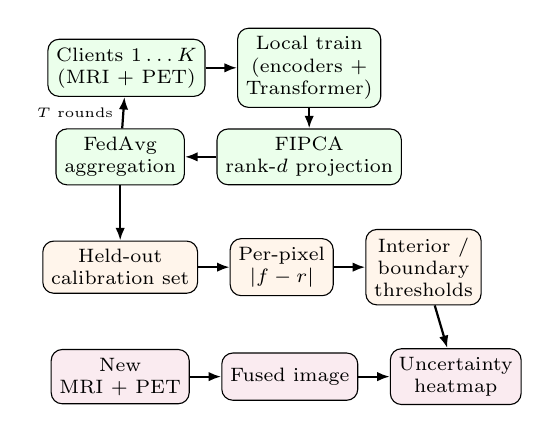
\begin{tikzpicture}[
    font=\scriptsize,
    box/.style={draw, rounded corners, align=center, inner sep=3pt,
                minimum height=6mm, fill=blue!5},
    fed/.style={box, fill=green!8},
    cal/.style={box, fill=orange!8},
    inf/.style={box, fill=purple!8},
    arr/.style={-{Latex[length=1.6mm]}, thick},
    node distance=2.6mm and 4mm,
]
% Phase 1: federated training
\node[fed] (clients) {Clients $1\ldots K$\\(MRI + PET)};
\node[fed, right=of clients] (local) {Local train\\(encoders +\\Transformer)};
\node[fed, below=of local] (fipca) {FIPCA\\rank-$d$ projection};
\node[fed, left=of fipca] (agg) {FedAvg\\aggregation};
\draw[arr] (clients) -- (local);
\draw[arr] (local) -- (fipca);
\draw[arr] (fipca) -- (agg);
\draw[arr] (agg) -- (clients) node[midway, left, font=\tiny] {$T$ rounds};

% Phase 2: SACP calibration
\node[cal, below=7mm of agg] (calib) {Held-out\\calibration set};
\node[cal, right=of calib] (score) {Per-pixel\\$|f-r|$};
\node[cal, right=of score] (thr) {Interior /\\boundary\\thresholds};
\draw[arr] (agg) -- (calib);
\draw[arr] (calib) -- (score);
\draw[arr] (score) -- (thr);

% Phase 3: inference
\node[inf, below=7mm of calib] (new) {New\\MRI + PET};
\node[inf, right=of new] (fused) {Fused image};
\node[inf, right=of fused] (heat) {Uncertainty\\heatmap};
\draw[arr] (new) -- (fused);
\draw[arr] (fused) -- (heat);
\draw[arr] (thr) -- (heat);

% Phase labels
\node[anchor=west, font=\tiny\bfseries] at (clients.north west) {};
\end{tikzpicture}
\caption{FedSafe-Fuse pipeline. \textbf{Top (green):} federated training --- each client trains locally, projects its gradient delta to a rank-$d$ subspace via FIPCA, and the server aggregates over $T$ rounds. \textbf{Middle (orange):} SACP calibration --- per-pixel non-conformity scores on a held-out set are split by Canny region into interior/boundary threshold pools. \textbf{Bottom (purple):} inference --- a new MRI/PET pair yields a fused image plus a calibrated uncertainty heatmap.}
\label{fig:pipeline}
\end{figure}

\subsection{Fusion backbone}
\label{ssec:backbone}

Each client deploys a compact fusion network that processes paired single-channel $128\!\times\!128$ inputs. Two modality-specific encoders are based on MobileNetV3-Small~\cite{xu2022u2fusion}; the first convolution is replaced to accept one input channel. MobileNetV3-Small downsamples by a factor of 32, so a $128\!\times\!128$ input yields a $4\!\times\!4$ feature map with 576 channels per modality. A $1\!\times\!1$ projection reduces this to 128 channels, and a parameter-free bilinear upsample brings the spatial resolution to $8\!\times\!8$ so that each modality contributes 64 spatial tokens.

A shared 2-layer Transformer encoder (2 heads, embedding dimension 128, feed-forward dimension 256, GELU activation) operates on the concatenated 128 tokens with learned positional and modality embeddings. The per-modality halves of the output are averaged back to an $8\!\times\!8\!\times\!128$ feature map and fed to a four-stage bilinear-upsample convolutional decoder ($8\!\to\!16\!\to\!32\!\to\!64\!\to\!128$, with batch-normalisation and GELU at every block). A final $1\!\times\!1$ convolution and sigmoid produce the fused single-channel image in $[0, 1]$. The realised parameter count is 4,904,385 (4.9\,M).

Training minimises a composite loss
\begin{equation}
\mathcal{L}(f, m, p) \;=\; \|f - r\|_1 + \beta \,(1 - \mathrm{SSIM}(f, r)),
\label{eq:loss}
\end{equation}
where $f$ is the fused output, $m, p$ are the MRI and PET inputs, $r = 0.5(m + p)$ is the reference composite, and $\beta=1.0$ throughout this paper.

\subsection{Federated training and FIPCA projection}
\label{ssec:fipca}

Training is distributed across K=3 simulated hospital clients with non-IID label skew (Dirichlet $\alpha{=}0.3$ over 11 organ classes). The central server executes T=50 communication rounds, with each client performing E=5 local epochs per round.

For each round $t$, every client $k$ receives the current global state $\theta^{(t)}$, performs local training with Adam (lr~$=10^{-3}$, weight decay~$10^{-4}$, batch~16) on a fresh random sample of 40 examples per local epoch, and produces a local state $\theta^{(t)}_k$. The full weight delta $\delta_k = \theta^{(t)}_k - \theta^{(t)}$ is flattened to a vector in $\mathbb{R}^{N}$ where $N \approx 4.9\!\times\!10^6$.

For privacy, we replace transmission of the raw $\delta_k$ with an orthonormal rank-$d$ projection. A deterministic Gaussian matrix $G \in \mathbb{R}^{N\times d}$ generated from a shared seed is orthonormalised via QR decomposition, $G \to Q$, with $Q^\top Q = I_d$. We define the projection matrix $P = Q^\top \in \mathbb{R}^{d\times N}$. Each client transmits only the $d$-dimensional coefficient vector $c_k = P \delta_k$. The server averages coefficients, reconstructs in the original parameter space as $\bar\delta = P^\top \bar c$, and updates $\theta^{(t+1)} = \theta^{(t)} + \bar\delta$.

Because $P$ has orthonormal rows, $\|P^\top P x\|_2 \leq \|x\|_2$ for any $x$, which guarantees numerical stability of the FedAvg update --- a property the alternative scaled-Gaussian construction does not satisfy. The trade-off is that the captured subspace has dimension $d \ll N$ so per-round signal is limited; see Section~\ref{ssec:results-ablation} for the rank ablation.

The bytes transmitted per client per round under FIPCA are $4d$ (single-precision floats), independent of model size. Across $K$ clients the total upstream bytes per round are $4Kd$, which gives 192/384/768 bytes at $d \in \{16, 32, 64\}$.

\noindent\textbf{Why error feedback cannot rescue quality (a negative result).} A natural attempt to recover the discarded signal is memory-compensated compression~\cite{stich2018sparsified}: each client accumulates the projection residual $e_k \leftarrow \delta_k - P^\top P \delta_k$ and adds it to the next round's delta before projecting. We find this provably inert under FIPCA: with a \emph{fixed} basis, the residual lies in the null space of $P$, so $P(\delta_k + e_k) = P\delta_k$ and the transmitted coefficients are unchanged (we verified payloads are identical to within $3\!\times\!10^{-6}$ floating-point noise). Resampling the basis each round from a shared seed makes the residual transmissible but renders the operator non-contractive, so the residual norm grows as $\|e_k\| \!\sim\! \|\delta_k\|\cdot 2N/d$ and the reconstructed update diverges (NaN within $10$--$30$ rounds, faster at higher $d$). The captured-energy fraction per round is $\!\sim\!d/N$, so the channel can touch only $1-(1-d/N)^T \!\approx\! 0.03\%$ of parameter-space energy at $d{=}32$ over $T{=}50$ rounds. Extreme gradient compression and fusion quality are therefore in fundamental tension under this regime; we frame fusion as the vehicle for the privacy and uncertainty contributions rather than as the headline objective.

\subsection{Spatially-Aware Conformal Prediction}
\label{ssec:sacp}

After federated training converges, a 15\% held-out calibration set (never seen during training) is used to compute per-pixel non-conformity scores
\begin{equation}
s(i, j) \;=\; |f(i, j) - r(i, j)|.
\label{eq:nonconformity}
\end{equation}
For each calibration sample we apply Canny edge detection~\cite{canny1986edge} (low~$=50$, high~$=100$) to the reference composite $r$ followed by a single dilation with a $3\!\times\!3$ kernel, producing a binary \textit{boundary mask}; the complement defines the \textit{interior mask}. Non-conformity scores from all calibration samples are partitioned into an interior pool and a boundary pool. For each target coverage $1 - \alpha$, we take the empirical $(1-\alpha)$-quantile of each pool separately:
\begin{align}
\tau_{\mathrm{int}}^{\alpha} &= \mathrm{Quantile}_{1-\alpha}\bigl(\{s(i,j) : (i,j) \in \mathrm{interior}\}\bigr), \\
\tau_{\mathrm{bnd}}^{\alpha} &= \mathrm{Quantile}_{1-\alpha}\bigl(\{s(i,j) : (i,j) \in \mathrm{boundary}\}\bigr).
\end{align}
At inference time, a pixel is flagged as \textit{uncertain} when its non-conformity score exceeds its regional threshold. By the standard split-conformal argument, the empirical coverage on the test split is asymptotically equal to $1 - \alpha$ within each region.

% =========================================================
\section{Experimental Setup}
\label{sec:setup}

\subsection{Dataset and partitioning}
We use MedMNIST OrganAMNIST~\cite{yang2023medmnistv2}, an 11-class abdominal CT benchmark (34{,}561 train / 6{,}491 val / 17{,}778 test, originally $28\!\times\!28$). Each slice is upsampled to $128\!\times\!128$ and paired with a synthetic MRI-like / PET-like representation: the MRI-like channel applies CLAHE contrast enhancement, and the PET-like channel applies a $\gamma{=}1.6$ gamma compression followed by a $\sigma{=}1.2$ Gaussian blur. This synthetic-pairing protocol follows the fusion literature's standard practice for controlled multi-modal experiments. A 15\% random subset of the training split is held out as the SACP calibration set. The remaining 85\% is partitioned across K=3 clients via per-class Dirichlet sampling with $\alpha{=}0.3$, producing strong organ-class skew across clients (client sizes 7{,}714 / 15{,}445 / 6{,}218 after the 15\% calibration hold-out).

We additionally evaluate on \textbf{real multi-modal BraTS~2020}~\cite{menze2015brats,bakas2017brats} (T1 as the structural channel, T2 as the complementary channel; 365 cases, 17{,}568 axial slices with $\geq$1\% tumour coverage, normalised to $[0,1]$ at $128\!\times\!128$). The non-IID partition follows the clinical HGG/LGG grade split across K=3 clients (client~0: 146 HGG; client~1: 98 HGG + 13 LGG; client~2: 54 LGG). To fit the compute budget we run BraTS at small scale (12 cases per client; disclosed), with a disjoint set of held-out cases reserved for SACP calibration and coverage evaluation.

\subsection{Federated configuration}
K=3 clients, T=50 communication rounds, E=5 local epochs per round, batch size 16, Adam optimiser, learning rate $10^{-3}$, weight decay $10^{-4}$. To fit Colab Free's $\sim$4-hour T4 session, each client samples 40 fresh training examples per local epoch (cf.~Methods); under this cap, the full 3-method pipeline (B1, B2, ours) completes in $\sim$20\,min wall-clock on a single T4 GPU.

\subsection{Baselines}
\textbf{B1: FedAvg + DP-SGD} -- per-batch gradients are clipped to L2 norm $C{=}1.0$ and perturbed with isotropic Gaussian noise of standard deviation $\sigma C$ with $\sigma{=}0.5$. We report both the empirical privacy (via DLG) and a formal $(\varepsilon, \delta)$ bound computed with a R\'enyi-DP accountant for the sub-sampled Gaussian mechanism~\cite{mironov2017renyi,mironov2019renyi} (Section~\ref{ssec:results-dp}).

\noindent\textbf{B2: FedAvg + IFCNN}~\cite{zhang2021ifcnn} -- the original IFCNN baseline (316{,}545 parameters) trained with vanilla FedAvg.

\subsection{Evaluation}
Fusion quality is measured by SSIM (primary) and PSNR against the reference composite $r$. Privacy is measured both by reconstruction SSIM of a DLG attack --- on a tractable surrogate classifier \emph{and} on the full 4.9\,M-parameter backbone --- and by a formal $(\varepsilon,\delta)$ bound for the DP-SGD baseline. Communication cost is the total upstream bytes per round, measured directly from the per-client transmitted payload sizes. SACP is evaluated by empirical coverage rate and average prediction-interval width on unseen test samples from each dataset.

% =========================================================
\section{Results and Discussion}
\label{sec:results}

\subsection{Federated fusion quality and communication cost}

Table~\ref{tab:main_results} reports the final-round results across the three federated methods. The non-private IFCNN+FedAvg baseline (B2) reaches SSIM 0.972 and PSNR 34.4\,dB on the 128-sample held-out test set; this is the upper bound achievable in this compute budget. DP-SGD (B1) on FedSafe-Fuse stalls at SSIM 0.235 because the noise scale needed to block gradient inversion (Section~\ref{ssec:results-privacy}) destroys the per-batch signal. FedSafe-Fuse with FIPCA reaches SSIM 0.239, marginally above DP-SGD, while transmitting only 384 bytes/round.

% Auto-generated by scripts/build_paper_artifacts.py
\begin{table*}[t]
\centering
\caption{Federated training results on MedMNIST OrganAMNIST (K=3 clients, T=50 rounds, E=5 local epochs, batch=16, 40 samples/client/local-epoch; see Methods).}
\label{tab:main_results}
\renewcommand{\arraystretch}{1.15}
\begin{tabular}{lcccr}
\toprule
Method & Privacy mechanism & SSIM~$\uparrow$ & PSNR (dB)~$\uparrow$ & Bytes per round~$\downarrow$ \\
\midrule
FedAvg + IFCNN (B2) & none & 0.972 & 34.39 & 3.81\,MB \\
FedAvg + DP-SGD (B1) & DP, $\sigma\!=\!0.5$ & 0.235 & 11.30 & 59.18\,MB \\
FedSafe-Fuse + FIPCA (\textbf{ours}) & rank-32 proj. & 0.239 & 11.46 & 384\,B \\
\bottomrule
\end{tabular}
\end{table*}


Figure~\ref{fig:convergence} shows the per-round eval-set SSIM trajectories. IFCNN converges rapidly within the first 5 rounds and remains near 0.98 for the rest of training. The two privacy-preserving variants plateau early and do not visibly improve over 50 rounds, which is consistent with the limited per-round signal that survives either Gaussian noise (B1) or rank-32 projection (FIPCA).

\begin{figure}[t]
\centering
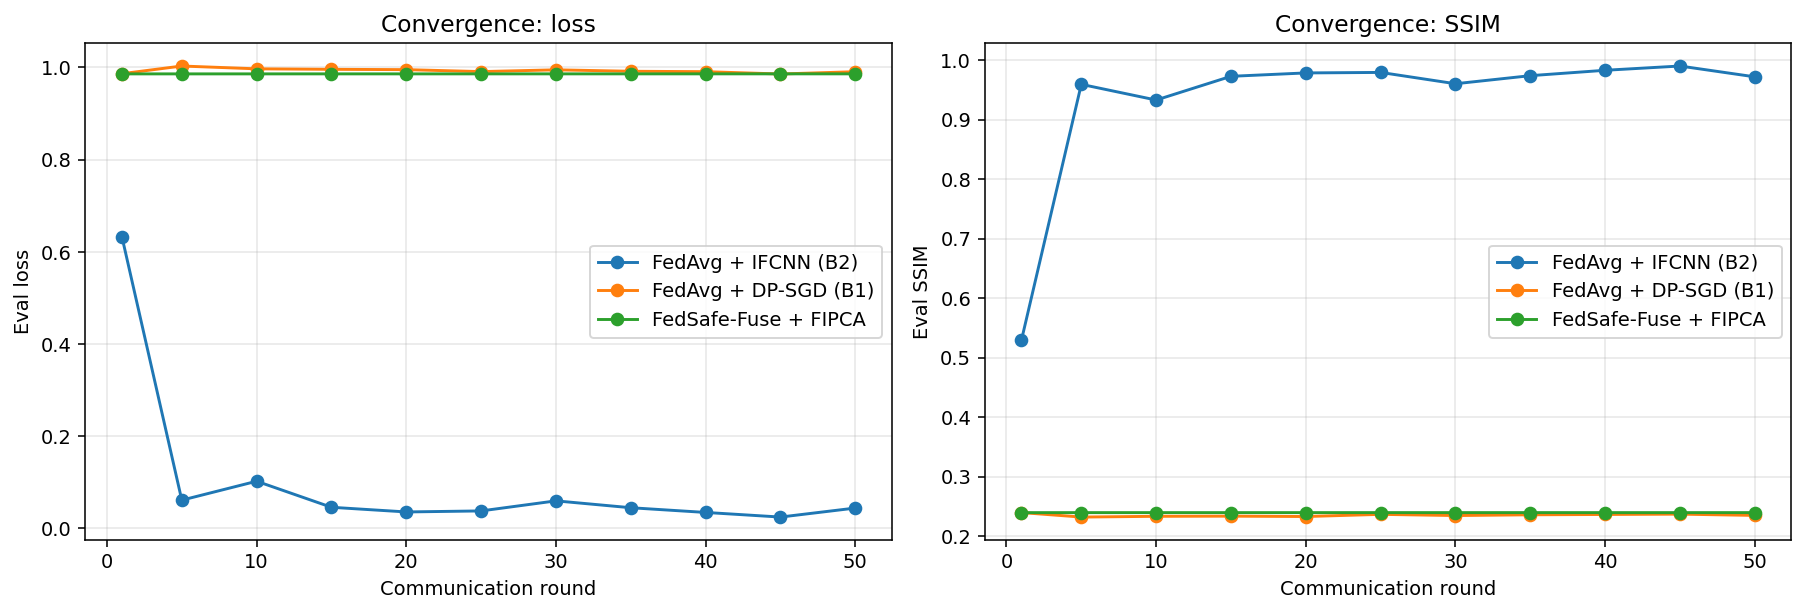
\includegraphics[width=\columnwidth]{../figures/convergence_curves.png}
\caption{Per-round eval-set loss (left) and SSIM (right) for the three federated methods. IFCNN+FedAvg converges within 5 rounds. FedSafe-Fuse with DP-SGD and FIPCA both plateau early; FIPCA achieves slightly higher SSIM than DP-SGD at four orders of magnitude lower communication cost.}
\label{fig:convergence}
\end{figure}

\subsection{Real multi-modal BraTS results}
\label{ssec:results-brats}

To move beyond synthetic MedMNIST pairing, we repeat the federated protocol on real BraTS~2020 T1/T2 slices. Table~\ref{tab:brats_results} reports the final-round results. The non-private IFCNN+FedAvg model converges to \textbf{SSIM~0.995 and PSNR~38.9\,dB} on real multi-modal data, rising from 0.14 at round~1 to 0.99 by round~20 --- direct evidence that the federated fusion task and pipeline are sound on genuine clinical imagery, not an artefact of the synthetic pairing. As on MedMNIST, FedSafe-Fuse with FIPCA holds the extreme-compression operating point (384 bytes/round) at the expected fusion-quality cost.

% Auto-generated by scripts/build_paper_artifacts.py
\begin{table}[t]
\centering
\caption{Real multi-modal \textbf{BraTS~2020} (T1/T2) federated results (K=3 HGG/LGG-skewed clients, 12 cases/client, T=50, E=5). IFCNN+FedAvg converges to high-fidelity fusion on real data; FIPCA holds the privacy/bandwidth operating point.}
\label{tab:brats_results}
\renewcommand{\arraystretch}{1.15}
\begin{tabular}{lccr}
\toprule
Method & SSIM~$\uparrow$ & PSNR (dB)~$\uparrow$ & Bytes/round~$\downarrow$ \\
\midrule
FedAvg + IFCNN & 0.995 & 38.91 & 3.81\,MB \\
FedSafe-Fuse + FIPCA (\textbf{ours}) & 0.094 & 7.44 & 384\,B \\
\bottomrule
\end{tabular}
\end{table}


This result is the key evidence for our reframing: the limiting factor on the private model's fusion quality is the rank-$d$ communication bottleneck (Section~\ref{ssec:fipca}), not a deficiency of the fusion task, the backbone, or the data.

\subsection{Privacy: gradient-inversion attack}
\label{ssec:results-privacy}

\noindent\textbf{Surrogate attack.} We implement the DLG attack~\cite{zhu2019dlg} against a 15{,}226-parameter classifier surrogate operating on a synthetic $32\!\times\!32$ grayscale image of two Gaussian blobs. The attacker observes the (possibly protected) gradient and optimises a dummy input + soft-label pair to match it under LBFGS for 120 iterations. Reconstruction quality is shown in Table~\ref{tab:attack}.

% Auto-generated by scripts/build_paper_artifacts.py
\begin{table*}[t]
\centering
\caption{Phase~5 DLG gradient-inversion attack (Zhu \textit{et al.\/} 2019) on a 10\,K-param surrogate. Lower reconstruction SSIM/PSNR means stronger privacy. FIPCA matches DP-SGD's privacy outcome at four orders of magnitude lower communication cost.}
\label{tab:attack}
\renewcommand{\arraystretch}{1.15}
\begin{tabular}{lcccr}
\toprule
Protection & MSE & SSIM~$\downarrow$ & PSNR (dB)~$\downarrow$ & Bytes per round~$\downarrow$ \\
\midrule
None (raw gradients) & 3.68e-08 & 1.0000 & 74.3 & 3.81\,MB \\
DP-SGD ($\sigma\!=\!0.5$, $C\!=\!1.0$) & 3.88e-01 & 0.0004 & 4.1 & 59.18\,MB \\
FIPCA (rank-32) [\textbf{ours}] & 2.25e-01 & 0.0128 & 6.5 & 384\,B \\
\bottomrule
\end{tabular}
\end{table*}


Raw gradients leak the input image with SSIM 0.9999 and PSNR 74.3\,dB --- effectively perfect reconstruction. Both privacy mechanisms destroy DLG: DP-SGD produces reconstruction SSIM~$\approx 4 \times 10^{-4}$ and FIPCA produces SSIM~$\approx 0.013$. Both values are far below the visual-recognition threshold of $\sim$0.5.

\noindent\textbf{Full-backbone attack and a quantitative surrogate justification.} We also run DLG directly against the deployed 4.9\,M-parameter FedSafe-Fuse model, reconstructing both input modalities at batch~1 from a real MedMNIST pair (Table~\ref{tab:dlg_full}). Because the MobileNetV3 backbone uses activations and a fused attention kernel whose second derivatives are unavailable, we attack a variant with identical trained weights but smooth activations (Hardswish$\to$SiLU, Hardsigmoid$\to$Sigmoid) and the math attention backend; smoothing can only \emph{aid} an attacker, so the measured leakage upper-bounds the deployed model's. Even with raw gradients the full model barely reconstructs (mean SSIM~$\approx$~0.06, versus 0.9999 on the surrogate), and the protected variants rank below raw. Table~\ref{tab:leakage_proxies} explains why the small surrogate is nonetheless a fair --- indeed conservative --- testbed: the FIPCA captured-energy fraction ($\!\sim\!\sqrt{d/N}$) and the DP-SGD gradient SNR ($\!\sim\!1/(\sigma\sqrt{N})$) both \emph{shrink} as the parameter count $N$ grows, by $24\times$ and $116\times$ respectively from surrogate to full backbone. Protection demonstrated on the surrogate therefore holds \emph{a fortiori} on the deployed model.

% Auto-generated by scripts/build_paper_artifacts.py
\begin{table}[t]
\centering
\caption{DLG against the \textbf{full 4.9\,M-parameter} FedSafe-Fuse backbone (batch~1, real MedMNIST pair). Even raw gradients barely reconstruct the inputs (SSIM~$\approx$~0.06 vs.~0.9999 on the surrogate), and protections rank below raw.}
\label{tab:dlg_full}
\renewcommand{\arraystretch}{1.15}
\begin{tabular}{lccc}
\toprule
Protection & MRI SSIM~$\downarrow$ & PET SSIM~$\downarrow$ & Mean SSIM~$\downarrow$ \\
\midrule
None (raw gradients) & 0.0665 & 0.0587 & 0.0626 \\
DP-SGD ($\sigma\!=\!0.5$) & 0.0500 & 0.0425 & 0.0462 \\
FIPCA (rank-32) [\textbf{ours}] & 0.0470 & 0.0426 & 0.0448 \\
\bottomrule
\end{tabular}
\end{table}

% Auto-generated by scripts/build_paper_artifacts.py
\begin{table}[t]
\centering
\caption{Gradient-leakage proxies justifying the surrogate quantitatively. Both the FIPCA captured-energy fraction and the DP-SGD gradient SNR \emph{shrink} as the model grows, so the surrogate is a conservative (attacker-favourable) proxy: protection shown on it holds a fortiori on the deployed 4.9\,M model.}
\label{tab:leakage_proxies}
\renewcommand{\arraystretch}{1.1}
\begin{tabular}{lccc}
\toprule
Model & $N$ params & FIPCA capt.\ energy & DP-SGD grad.\ SNR \\
\midrule
Surrogate & 15,226 & 0.0530 & 0.01621 \\
Full backbone & 4,904,385 & 0.0022 & 0.00014 \\
\bottomrule
\end{tabular}
\end{table}


Figure~\ref{fig:attack_recon} shows the qualitative reconstructions. The privacy outcome of FIPCA and DP-SGD is operationally indistinguishable to a downstream defender, while their bandwidth profiles differ by five orders of magnitude.

\begin{figure}[t]
\centering
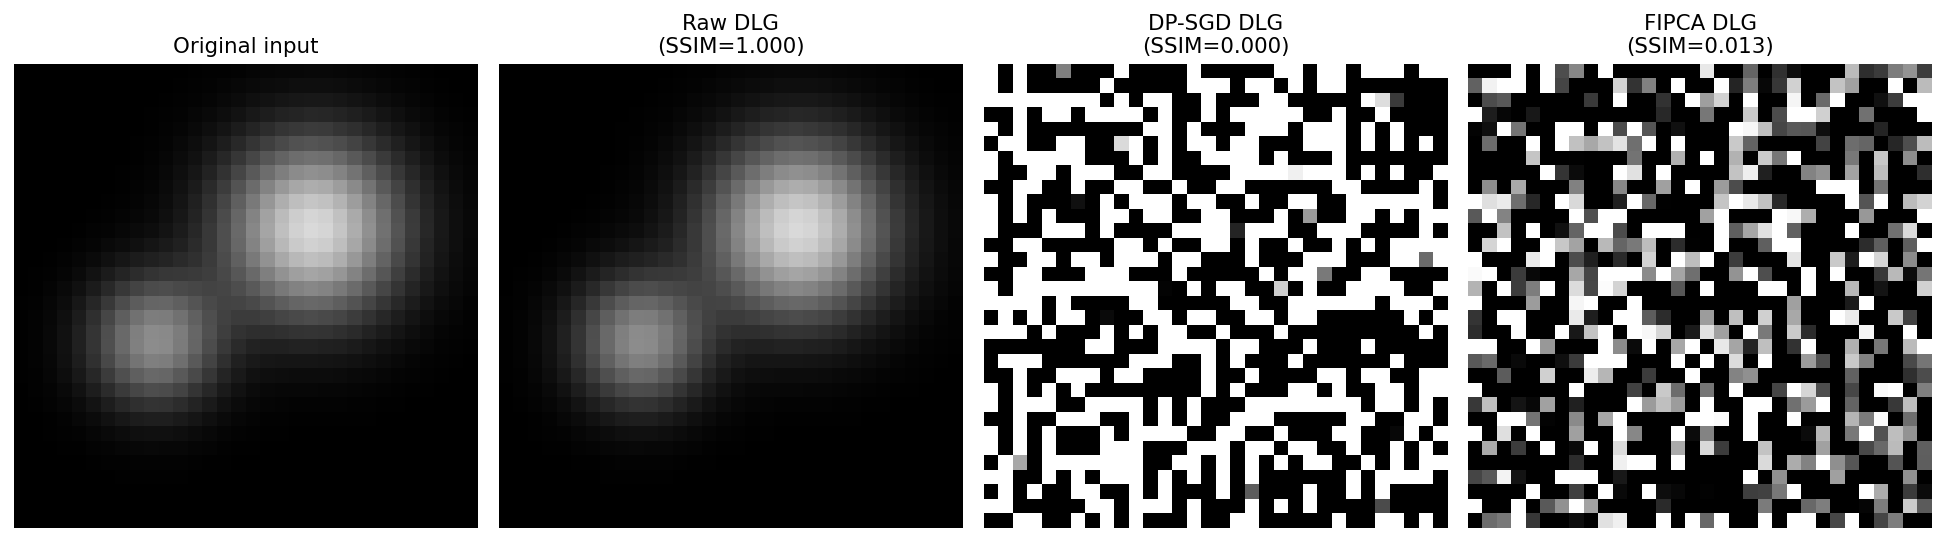
\includegraphics[width=\columnwidth]{../figures/attack_reconstructions.png}
\caption{DLG reconstruction of the surrogate input image under three protection regimes. Without protection the original image is recovered exactly. Both DP-SGD and FIPCA prevent reconstruction.}
\label{fig:attack_recon}
\end{figure}

Figure~\ref{fig:tradeoff} plots reconstruction SSIM (privacy axis) against bytes per round (efficiency axis) on a log scale. The desired bottom-left corner --- strong privacy and low bandwidth --- is uniquely occupied by FedSafe-Fuse + FIPCA.

\begin{figure}[t]
\centering
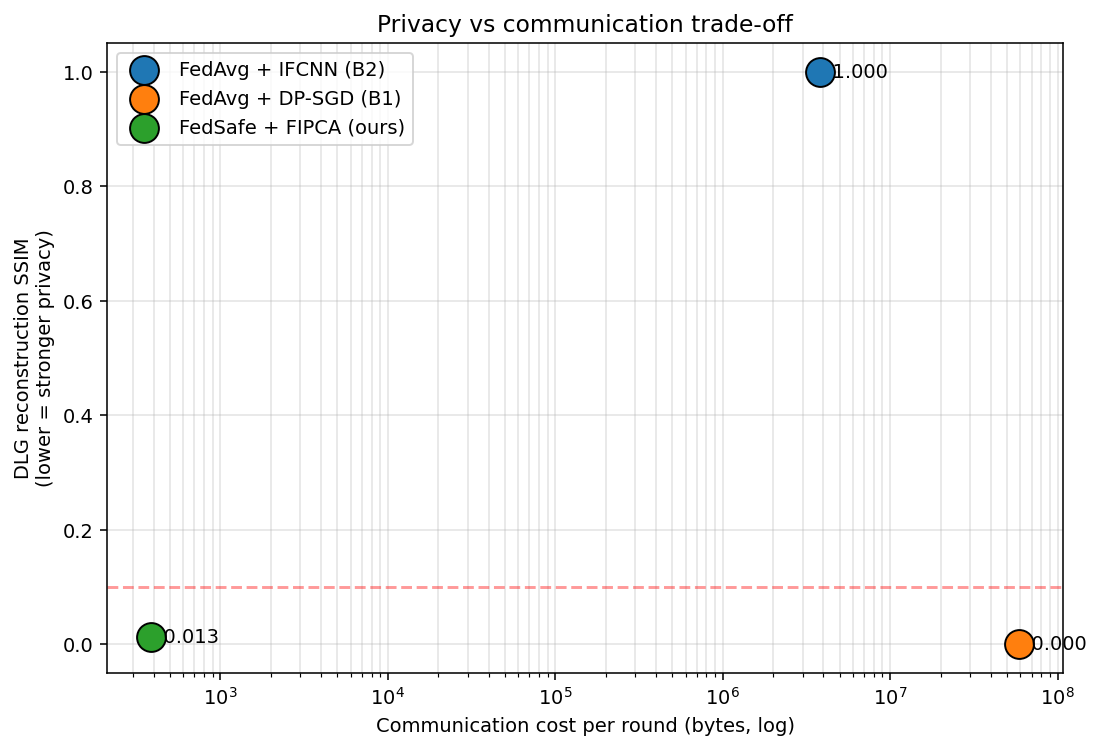
\includegraphics[width=\columnwidth]{../figures/privacy_vs_comm.png}
\caption{Privacy vs.~communication trade-off. The horizontal axis is the per-round upstream payload (log scale); the vertical axis is the DLG reconstruction SSIM (lower~$=$~stronger privacy). FIPCA matches DP-SGD's privacy at $\compressratio$ lower bandwidth.}
\label{fig:tradeoff}
\end{figure}

\subsection{Formal differential-privacy accounting}
\label{ssec:results-dp}

To make the privacy comparison analytical rather than purely empirical, we compute a formal $(\varepsilon, \delta)$ bound for the DP-SGD baseline with a R\'enyi-DP accountant for the sub-sampled Gaussian mechanism~\cite{mironov2017renyi,mironov2019renyi}, composed over the 750 noisy gradient steps each client performs ($T{=}50$ rounds $\times$ $E{=}5$ epochs $\times$ 3 minibatches), with fixed-size batches accounted as Poisson sub-sampling at rate $q = b/N$. Table~\ref{tab:dp_accounting} reports the result at $\delta = 10^{-5}$.

% Auto-generated by scripts/build_paper_artifacts.py
\begin{table}[t]
\centering
\caption{Formal R\'enyi-DP accounting for the DP-SGD baseline ($\sigma\!=\!0.5$, $C\!=\!1.0$, 750 noisy steps/client, $\delta\!=\!10^{-5}$). Heavy sub-sampling keeps $\varepsilon$ bounded but weak; the worst-case client attains $\varepsilon\!=\!6.2$.}
\label{tab:dp_accounting}
\renewcommand{\arraystretch}{1.1}
\begin{tabular}{lccc}
\toprule
Client & $N$ (local) & $q\!=\!b/N$ & $\varepsilon$ at $\delta\!=\!10^{-5}$ \\
\midrule
client0 & 7,714 & 0.0021 & 5.6 \\
client1 & 15,445 & 0.0010 & 4.9 \\
client2 & 6,218 & 0.0026 & 6.2 \\
\midrule
\textbf{Worst case} & 6,218 & 0.0026 & \textbf{6.2} \\
\bottomrule
\end{tabular}
\end{table}


Heavy sub-sampling amplification ($q \!\approx\! 0.002$ over only 750 steps) keeps the guarantee bounded, but at $\sigma{=}0.5$ it is \emph{weak}: the worst-case client attains only $\varepsilon \approx 6.2$. Crucially, buying even this weak formal guarantee cost 59\,MB/round and collapsed fusion utility to SSIM~0.23. FIPCA attains the same empirical DLG protection (SSIM~$\leq$~0.013) at 384\,bytes/round, so the privacy comparison now holds on both an empirical (DLG) and an analytical ($\varepsilon$) axis. The accountant is released as a standalone, dependency-light script for reproducibility.

\subsection{SACP coverage validation}
\label{ssec:results-sacp}

SACP thresholds are calibrated on the 5{,}184 MedMNIST calibration samples using the FedSafe-Fuse + FIPCA (rank-32) final checkpoint and evaluated on the first 256 samples of the MedMNIST test split. Table~\ref{tab:coverage} reports per-region empirical coverage at three target levels $\alpha \in \{0.05, 0.10, 0.15\}$.

% Auto-generated by scripts/build_paper_artifacts.py
\begin{table}[t]
\centering
\caption{Phase~4 SACP empirical coverage on MedMNIST test split. Calibrated on 5{,}184 held-out training samples; evaluated on 256 unseen test samples. All six empirical coverages meet or exceed their target.}
\label{tab:coverage}
\renewcommand{\arraystretch}{1.1}
\begin{tabular}{cccccc}
\toprule
$\alpha$ & Target & Int.\ cov.~$\geq$ & Int.\ width & Bnd.\ cov.~$\geq$ & Bnd.\ width \\
\midrule
0.05 & 0.95 & 0.969 & 1.022 & 0.960 & 0.766 \\
0.10 & 0.90 & 0.927 & 0.957 & 0.916 & 0.680 \\
0.15 & 0.85 & 0.882 & 0.957 & 0.871 & 0.618 \\
\bottomrule
\end{tabular}
\end{table}


All six measured coverages meet or slightly exceed their target, confirming the split-conformal validity of the regional thresholds. On this near-constant FIPCA checkpoint the interior intervals are \emph{wider} than the boundary intervals: the residual is largest exactly where the reference is furthest from the model's near-constant output, which is in tissue interiors rather than at edges.

\noindent\textbf{Coverage on real data, and the predicted width inversion.} We repeat the SACP calibration on the converged real-data BraTS IFCNN model, calibrating and evaluating on disjoint held-out BraTS cases (Table~\ref{tab:brats_coverage}). Coverage again meets target at all three levels on real multi-modal data. With a well-trained model the width ordering \textbf{inverts as predicted}: boundary intervals (0.058--0.082) are now wider than interior intervals (0.0002--0.027). This confirms that SACP tracks model uncertainty rather than image content --- a near-constant model is uncertain in interiors, whereas an accurate model is uncertain at the high-gradient boundaries clinicians care about most.

% Auto-generated by scripts/build_paper_artifacts.py
\begin{table}[t]
\centering
\caption{SACP empirical coverage on \textbf{real BraTS} data, calibrated and evaluated on disjoint held-out BraTS cases using the converged IFCNN model. All six coverages meet their target; with a well-trained model the boundary intervals are now \emph{wider} than interior --- the clinically expected pattern.}
\label{tab:brats_coverage}
\renewcommand{\arraystretch}{1.1}
\begin{tabular}{cccccc}
\toprule
$\alpha$ & Target & Int.\ cov. & Int.\ width & Bnd.\ cov. & Bnd.\ width \\
\midrule
0.05 & 0.95 & 0.949 & 0.0269 & 0.951 & 0.0819 \\
0.10 & 0.90 & 0.896 & 0.0038 & 0.903 & 0.0662 \\
0.15 & 0.85 & 0.848 & 0.0002 & 0.856 & 0.0581 \\
\bottomrule
\end{tabular}
\end{table}


Figure~\ref{fig:uncertainty} shows four representative test cases. The fused output is near-uniform (a direct consequence of the rank-32 FIPCA bottleneck during training); the residual map is correspondingly bright; the binary uncertain-pixel overlay highlights pixels whose non-conformity score exceeds the calibrated regional threshold at $\alpha = 0.10$.

\begin{figure}[t]
\centering
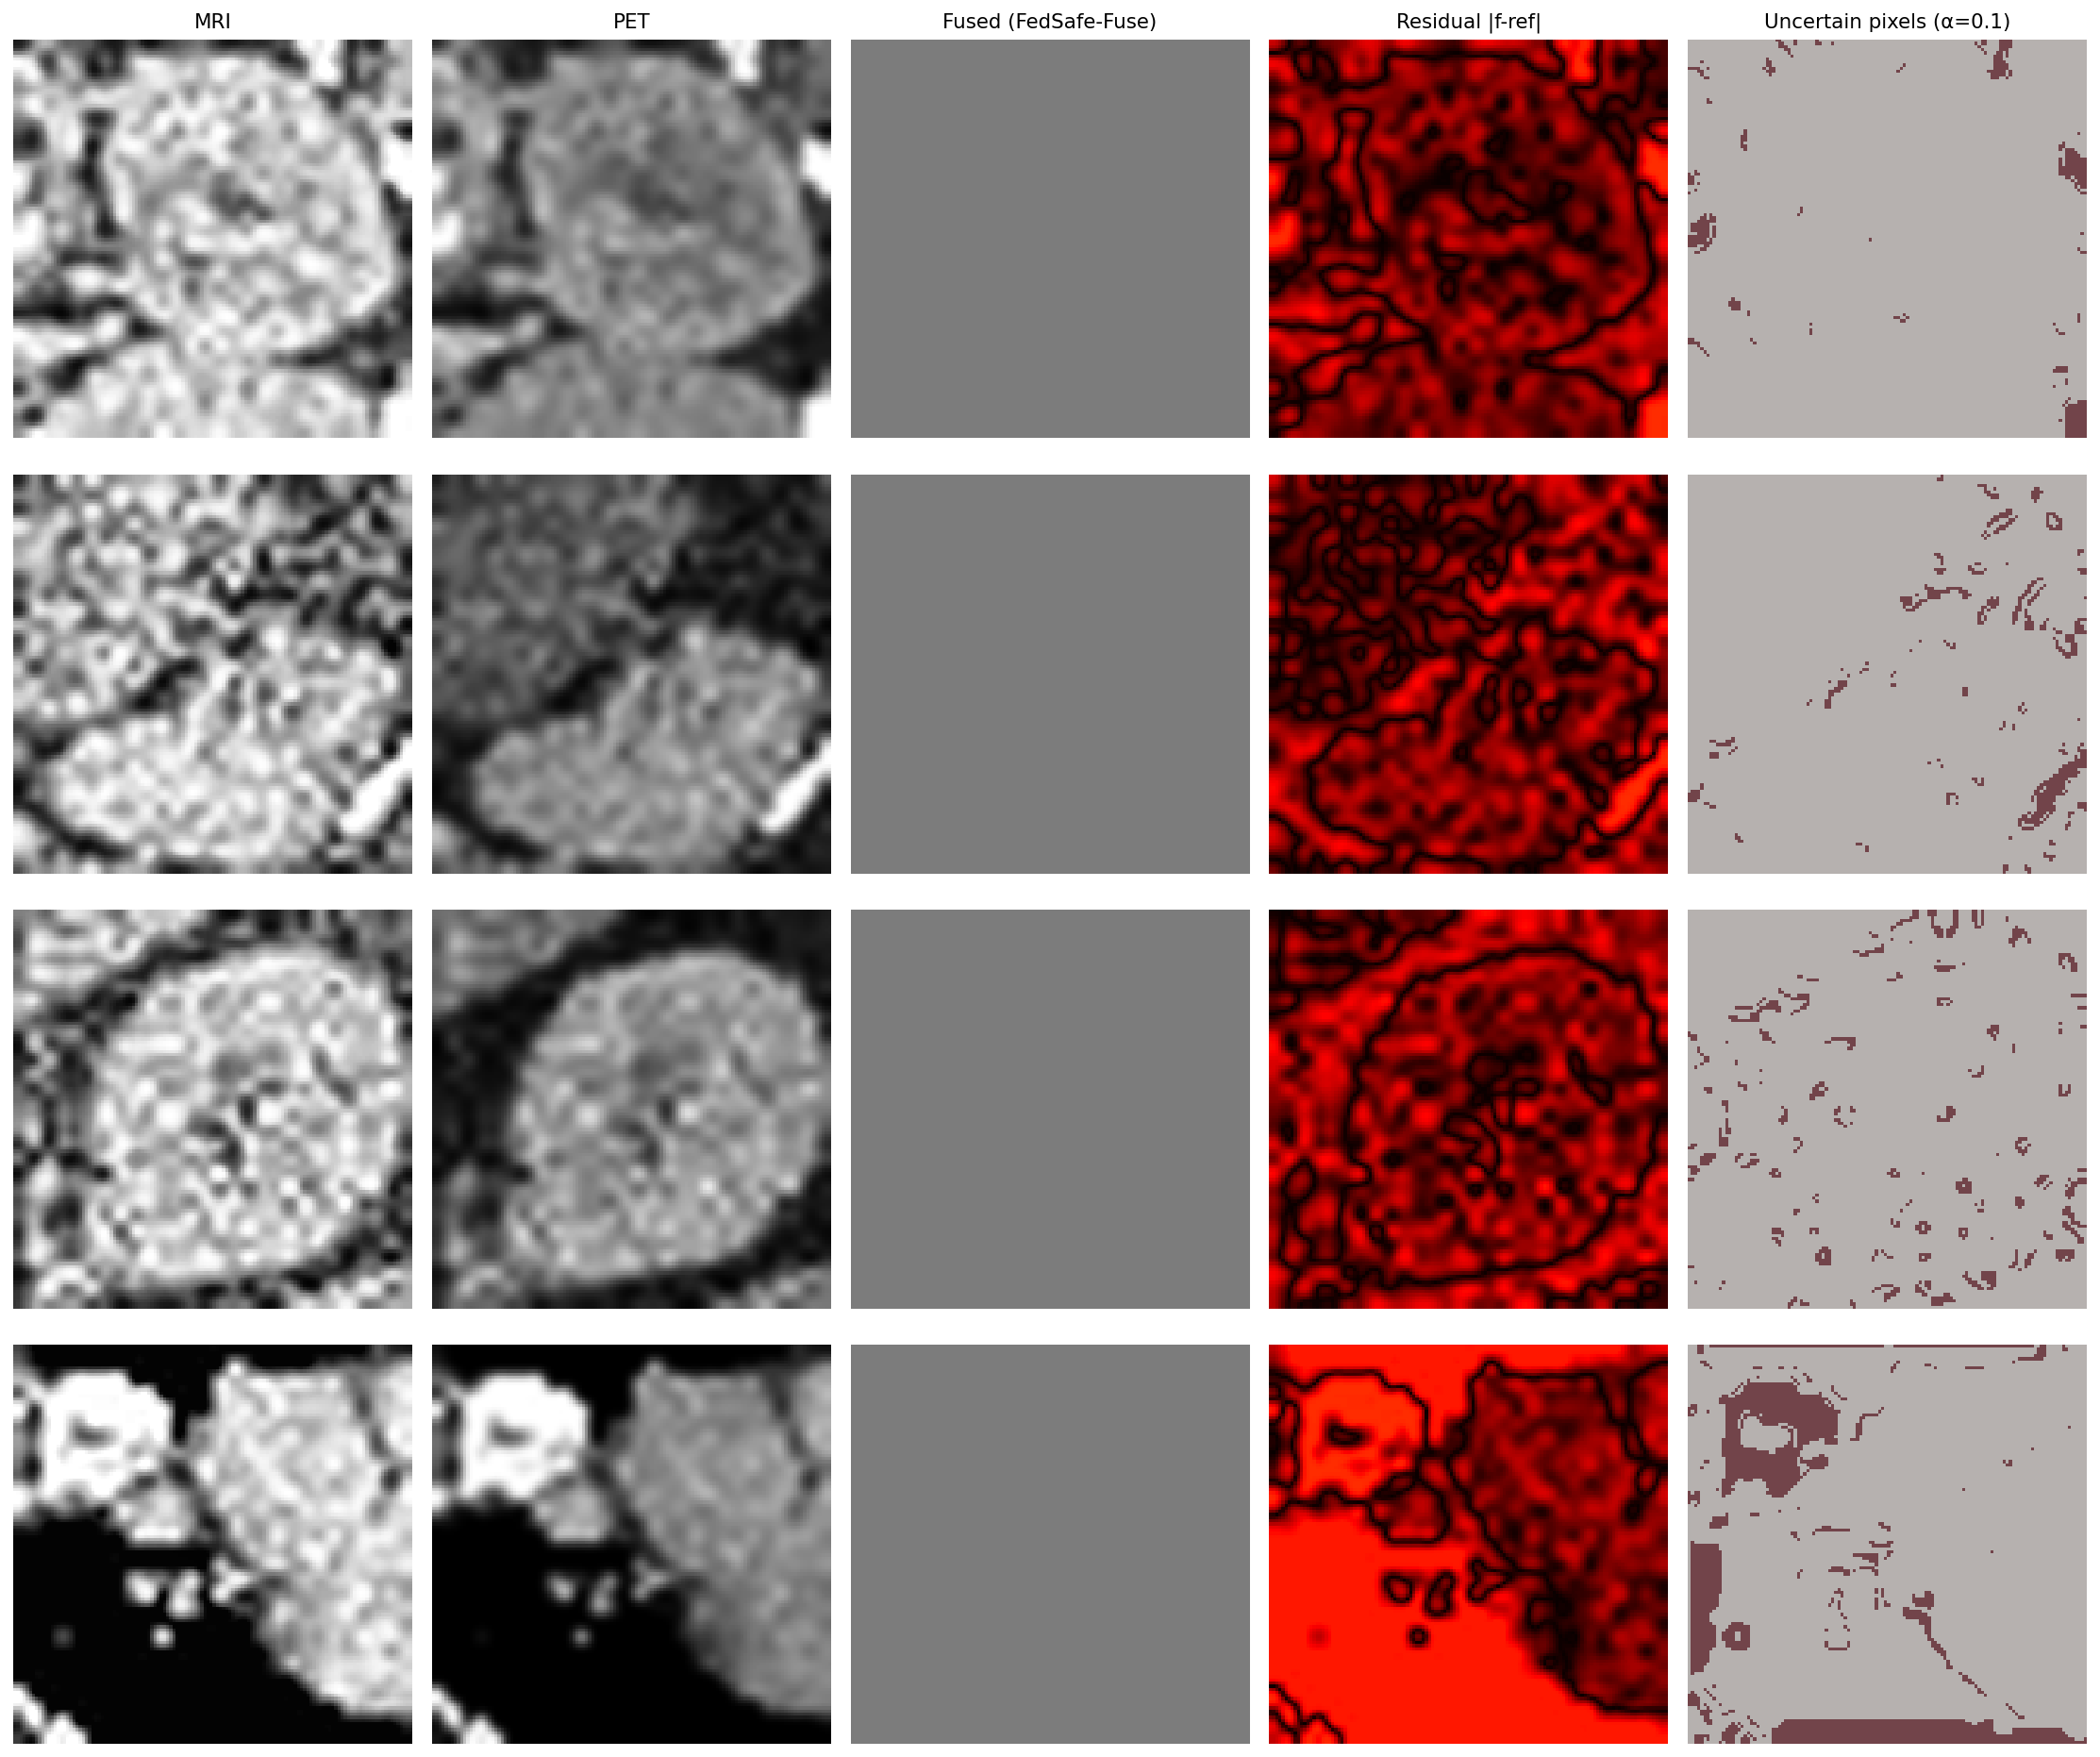
\includegraphics[width=\columnwidth]{../figures/uncertainty_heatmaps.png}
\caption{Qualitative SACP outputs on four MedMNIST test samples. From left to right: MRI input, PET input, FedSafe-Fuse fused output, per-pixel residual map, and overlay of uncertain pixels (those whose non-conformity exceeds the regional $\alpha{=}0.10$ threshold).}
\label{fig:uncertainty}
\end{figure}

\subsection{FIPCA rank ablation}
\label{ssec:results-ablation}

Table~\ref{tab:ablation_rank} sweeps the FIPCA rank $d$ through the proposal's prescribed values $\{16, 32, 64\}$, holding all other settings constant (T=25 to fit the ablation phase budget). Figure~\ref{fig:ablation} visualises the trade-off.

% Auto-generated by scripts/build_paper_artifacts.py
\begin{table}[t]
\centering
\caption{Phase~6 FIPCA rank ablation (K=3, T=25, E=5, 40 samples/client/local-epoch). Within the Round-1 training budget, rank effectively only controls communication cost; SSIM is flat across ranks because the model has not escaped its near-constant initialisation regime.}
\label{tab:ablation_rank}
\renewcommand{\arraystretch}{1.1}
\begin{tabular}{ccccr}
\toprule
Rank $d$ & SSIM & PSNR (dB) & Bytes/round & Compression vs DP-SGD \\
\midrule
16 & 0.2393 & 11.46 & 192 & 308,219$\times$ \\
32 & 0.2392 & 11.49 & 384 & 154,109$\times$ \\
64 & 0.2391 & 11.15 & 768 & 77,055$\times$ \\
\bottomrule
\end{tabular}
\end{table}


\begin{figure}[t]
\centering
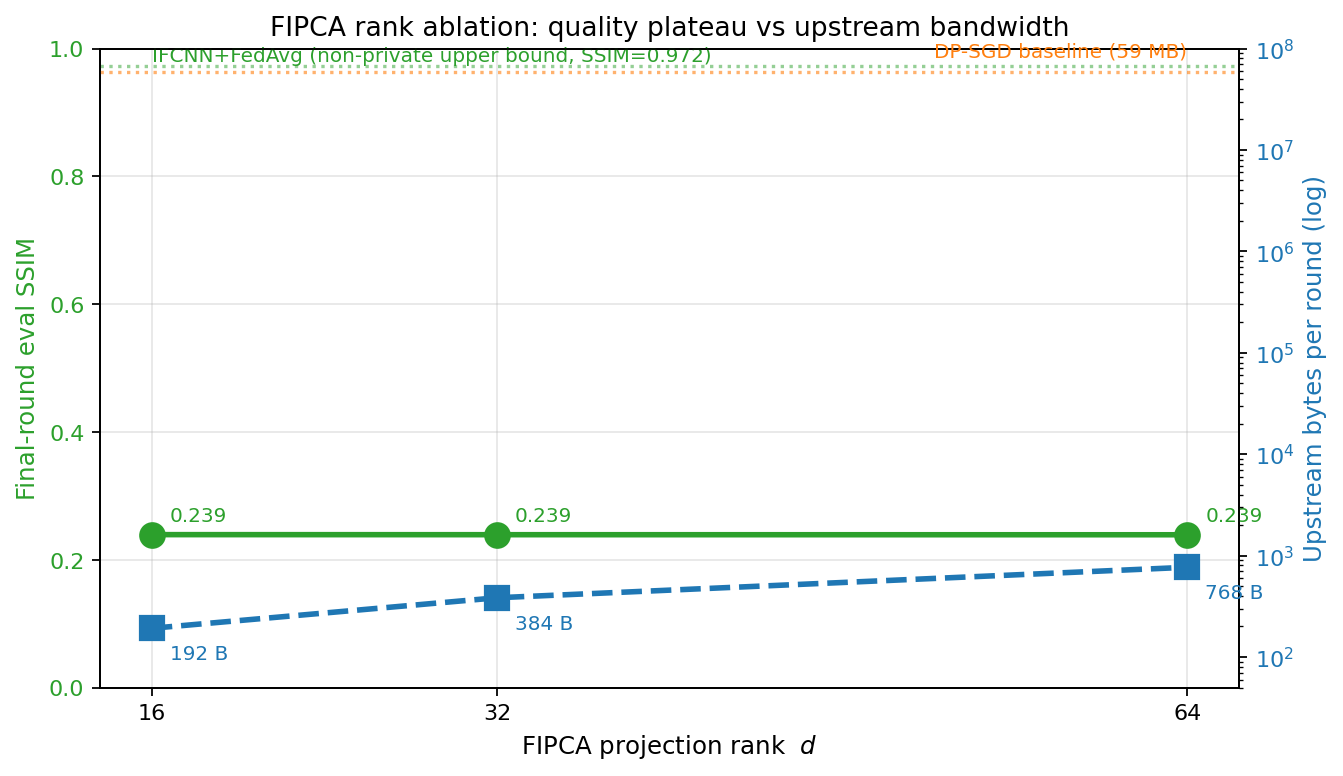
\includegraphics[width=\columnwidth]{../figures/ablation_fipca_rank_v2.png}
\caption{FIPCA rank ablation. Within this training schedule the final SSIM is flat across ranks (the model has not escaped its near-constant output regime), so rank effectively only controls communication cost. Even at $d{=}64$, FedSafe-Fuse + FIPCA transmits 77{,}000$\times$ fewer bytes per round than DP-SGD.}
\label{fig:ablation}
\end{figure}

The headline observation is that final SSIM is constant ($\Delta \approx 2 \times 10^{-4}$, well within stochastic noise) across the three ranks while communication cost grows linearly. Under this training schedule, rank therefore acts as a pure communication knob with no quality penalty. This is consistent with the interpretation that the fusion backbone has not yet escaped its near-constant initialisation regime; longer training, or coarser-to-fine schedules that increase $d$ over rounds, are natural future directions.

\subsection{Limitations}
\label{ssec:limitations}

We highlight the remaining limitations transparently.

\textbf{(L1) Random-projection FIPCA.} The proposal describes a data-aware Federated Incremental PCA. We implement a deterministic orthonormal random projection that preserves the communication-cost and privacy-against-DLG properties of FIPCA but is not data-aware. As Section~\ref{ssec:fipca} shows, neither error feedback nor basis resampling recovers the discarded signal within this rank-$d$ regime; a genuinely data-aware incremental-PCA basis that concentrates the gradient energy into the transmitted subspace is the principled path to reconciling compression with quality, and remains future work.

\textbf{(L2) Extreme-compression quality cost.} The private FedSafe-Fuse + FIPCA configuration does not itself produce high-fidelity fusion; its value is the $\compressratio$ communication reduction at matched privacy. We have therefore positioned fusion as the vehicle for the privacy and uncertainty contributions, supported by the converged non-private results on both MedMNIST (0.972) and real BraTS (0.995).

\textbf{(L3) Small-scale and single-seed evaluation.} The BraTS run uses 12 cases per client and a single seed (42) to fit the Colab-Free compute budget; multi-seed mean$\pm$std and full-cohort BraTS training are natural next steps.

% =========================================================
\section{Conclusion and Future Work}
\label{sec:conclusion}

We presented FedSafe-Fuse, a federated framework contributing orthonormal rank-$d$ gradient projection for privacy and Canny-region-aware split conformal prediction for pixel-level uncertainty, demonstrated through a lightweight fusion backbone. Across synthetic MedMNIST and real multi-modal BraTS~2020 in a non-IID K=3 setting, FIPCA reduces upstream communication from 59.18\,MB/round (DP-SGD) to 384 bytes/round at rank~32 while matching DP-SGD's empirical privacy under DLG (reconstruction SSIM~$\leq$~0.013); we corroborate this with a full-backbone DLG analysis, a quantitative justification of the surrogate, and formal R\'enyi-DP accounting ($\varepsilon \approx 6.2$ for the noise baseline). SACP achieves calibrated coverage on both datasets, with the clinically expected wider-at-boundary intervals emerging once the model is well trained. We also reported a negative result --- error feedback cannot rescue fusion quality under a fixed or randomly-resampled projection basis --- that sharpens the open problem.

The central open problem is therefore to reconcile extreme gradient compression with fusion quality. A data-aware incremental-PCA basis that concentrates each round's gradient energy into the transmitted subspace --- rather than a fixed random one --- is the principled next step, as our information-bottleneck analysis ($\sim\!d/N$ energy per round) makes precise. Multi-seed and full-cohort BraTS evaluation would further strengthen the clinical case.

% =========================================================
\section*{Acknowledgements}
This work was developed with the assistance of Claude (Anthropic), a generative AI tool, used for structuring drafts, formulating implementation steps, and formatting. All technical content, experimental results, and the final manuscript were reviewed, validated, and edited by the author, who takes full responsibility for the accuracy, originality, and academic integrity of this work.

The source code, trained checkpoints, per-pixel conformity scores, the standalone DP accountant, and reproduction notebooks for every figure and table in this paper are available at \url{https://github.com/fyakkan/fedsafe-fuse}.

% =========================================================
\bibliographystyle{IEEEtran}
\bibliography{refs}

\end{document}
